% Generated by scripts/paper_tex.py from paper-en.html; edit the HTML source (web/app/paper_src), not this file.
\documentclass[twocolumn]{aastex631}
\usepackage{xeCJK}
\setCJKmainfont{Noto Serif CJK TC}[BoldFont={Noto Serif CJK TC Bold}]
\setCJKsansfont{Noto Sans CJK TC}
\setCJKmonofont{Noto Sans Mono CJK TC}
\xeCJKsetup{CJKspace=true}
\usepackage{graphicx}
\usepackage{tabularx}

\shorttitle{Moving objects in SPHEREx images}
\shortauthors{SPHEREx Sky Change}
\begin{document}
\title{Finding moving objects in SPHEREx all-sky spectral imaging with a simulation-trained real/bogus network and parallax linking}
\author{SPHEREx Sky Change Team}
\affiliation{NASA Space Apps Challenge 2026 · Planet X and SPHEREx}
\begin{abstract}
SPHEREx maps the whole sky every six months in 102 near-infrared bands, which makes it a new tool for finding things that move: asteroids, comets and, in principle, a distant undiscovered planet. Its design also makes change detection hard. Each detector carries a linear variable filter, so the wavelength changes across the field; the point-spread function is undersampled (FWHM $\approx$ 5$''$ on 6.15$''$ pixels); and consecutive images of the same sky are taken at different wavelengths. We built a pipeline that (i) resamples every exposure of a 0.5$^\circ$ patch onto one sky grid, (ii) builds a reference for each pixel from exposures of the same detector whose wavelength at that pixel is within 3\% and that are at least 3 h away, (iii) detects 5$\sigma$ positive residuals, (iv) scores each candidate with a convolutional network, and (v) links detections into straight-line tracks or, across survey passes, into Earth-parallax tracks. The network never saw a real asteroid during training: it learned from movers injected with the instrument's own PSF and from real artifacts. In 19 fields it never trained on, it separates 556 detections of real known asteroids from false signals in the same fields with AUROC 0.987 (95\% CI 0.981--0.992), keeping 90.8\% of them at a false-positive rate of 1.15\%. Matched detections agree with JPL predictions for the spacecraft to a median 0.7$''$. The per-exposure 50\% completeness for injected movers is AB 17.3. Injected distant bodies on circular orbits were recovered from parallax plus a fitted orbital motion in 47/48 cases in fields with three survey passes (and, by construction, in none of a two-pass field); an earlier version that ignored orbital motion in both the injections and the fit was circular, and we report it as such. We report two failures that mattered: a noise model that capped real movers at S/N $\approx$ 10, and a pipeline flag that is set on real movers but never on simulated ones. From SPHEREx parallax alone, a blind search measured the distances of two real dwarf planets: Makemake 52.71 AU (JPL 52.72, 0.02\% off) and Haumea 49.49 AU (JPL 49.82, 0.66\%). A search of 32 fields (7.89 deg$^2$) along the predicted path of Planet Nine and around the 2025 IRAS/AKARI candidate found no distant track in single exposures; shift-and-stack (50\% completeness AB 19.2) linked 63 tracks, as many as chance produces when the survey-pass times are relabelled (55 and 60). We did not find a new planet; the injection tests and this non-detection show what the method can and cannot reach.

\medskip\noindent\textbf{Key points}
\begin{itemize}\setlength{\itemsep}{1pt}
\item A difference-imaging pipeline built for SPHEREx's linear variable filter matches references pixel by pixel in wavelength and detects moving sources in single 2-minute exposures.
\item A 0.32 M-parameter CNN trained only on injected movers separates 556 detections of real known asteroids in 19 fields it never trained on from false signals in the same fields with AUROC 0.987; signal-to-noise alone gives 0.537.
\item Fitting distance and orbital motion together across survey passes recovered 47 of 48 injected distant bodies (500--3000 AU) moving on circular orbits in fields with three survey passes (none in a two-pass field), with a median distance error of 0.09\%.
\item Positions of known asteroids agree with JPL Horizons predictions computed for the SPHEREx spacecraft to a median of 0.7$''$ (0.11 px, 78 detections of 6 objects).
\end{itemize}
\noindent{\footnotesize Hackathon technical report, not peer reviewed. Website and data: \url{https://quilt-advocate-boys-recovered.trycloudflare.com}}
\end{abstract}
\keywords{Asteroids --- Trans-Neptunian objects --- Astronomy image processing --- Convolutional neural networks --- Parallax}


\section{Introduction}
\label{sec:intro}
The 2026 Space Apps challenge asks for a public web tool that shows SPHEREx images of the sky and makes it easy to see how they change. Asteroids, comets, nearby stars, brown dwarfs and possibly new planets betray themselves by moving between images. Projects such as Backyard Worlds (Kuchner et al., 2017) showed that the public can find moving objects in WISE data by blinking images. SPHEREx (Doré et al., 2014) offers a richer data set, but blinking its raw images is misleading: two images of the same star taken at different wavelengths look different even when nothing has moved.

We therefore put a measured detection pipeline behind the public viewer, so that what people are shown has already passed quantitative tests. We set out to test three hypotheses (their criteria and when they were fixed are listed in Appendix A):

\begin{itemize}
\item \textbf{H1.} A network trained only on simulated movers recognises real known asteroids with AUROC $\ge$ 0.95.
\item \textbf{H2.} Per-pixel wavelength matching plus a reference-flux error term keeps the false-positive rate at the chosen operating point low in every detector.
\item \textbf{H3.} Earth's parallax between survey passes measures the distance of injected distant bodies to within 2\%.
\end{itemize}

\section{Data}
\label{sec:data}
We used SPHEREx Quick Release level-2 spectral images (collections \texttt{spherex\_qr2} and \texttt{spherex\_qr3}) from NASA/IPAC IRSA, spanning May 2025 to September 2026: three all-sky passes and part of a fourth. Each exposure covers about 3.5$^\circ$ $\times$ 3.5$^\circ$ with one of six detectors (D1--D6, 0.75--5.0 $\mu$m). We requested cutouts through IRSA's image-cutout service and used the IMAGE (minus ZODI), VARIANCE and FLAGS extensions, the per-pixel wavelength table (\texttt{WAVE-TAB} WCS) and the PSF cube (11 $\times$ 11 detector zones, 10$\times$ oversampled). QR3 files carry an \texttt{EPSF} table instead of the cube; for injections into QR3 exposures we reused a QR2 cube of the same detector.

Sixteen 0.5$^\circ$ fields sample the ecliptic every 30$^\circ$ in longitude ($\beta$ = 0$^\circ$ or 3$^\circ$), plus four at |$\beta$| = 12$^\circ$. Fifteen more fields were centred on asteroids with 13 $\le$ V $\le$ 17 found with the JPL Small-Body Identification API at the ecliptic longitude SPHEREx was observing on six dates; they are used only for evaluation. Known objects for every visit (exposures within 0.5 d) come from the same API (V $\le$ 21.5), with positions propagated linearly within the visit.

\begin{table*}[t]
\centering
\footnotesize

\begin{tabular}{llllll}
\hline\hline
Role & Fields & Candidates & Injected & Known asteroids (V$\le$18.5) & Bogus \\
\hline
Train & 12 & 729,286 & 12,351 & 199 & 716,736 \\
Validation & 2 & 68,573 & 2,227 & 27 & 66,319 \\
Test & 2 & 75,834 & 2,881 & 42 & 72,911 \\
Bright-asteroid benchmark & 15 & 428,053 & 0 & 487 & 427,566 \\
\hline
\end{tabular}
\end{table*}
\section{Methods}
\label{sec:methods}
\begin{figure}[t]
\centering
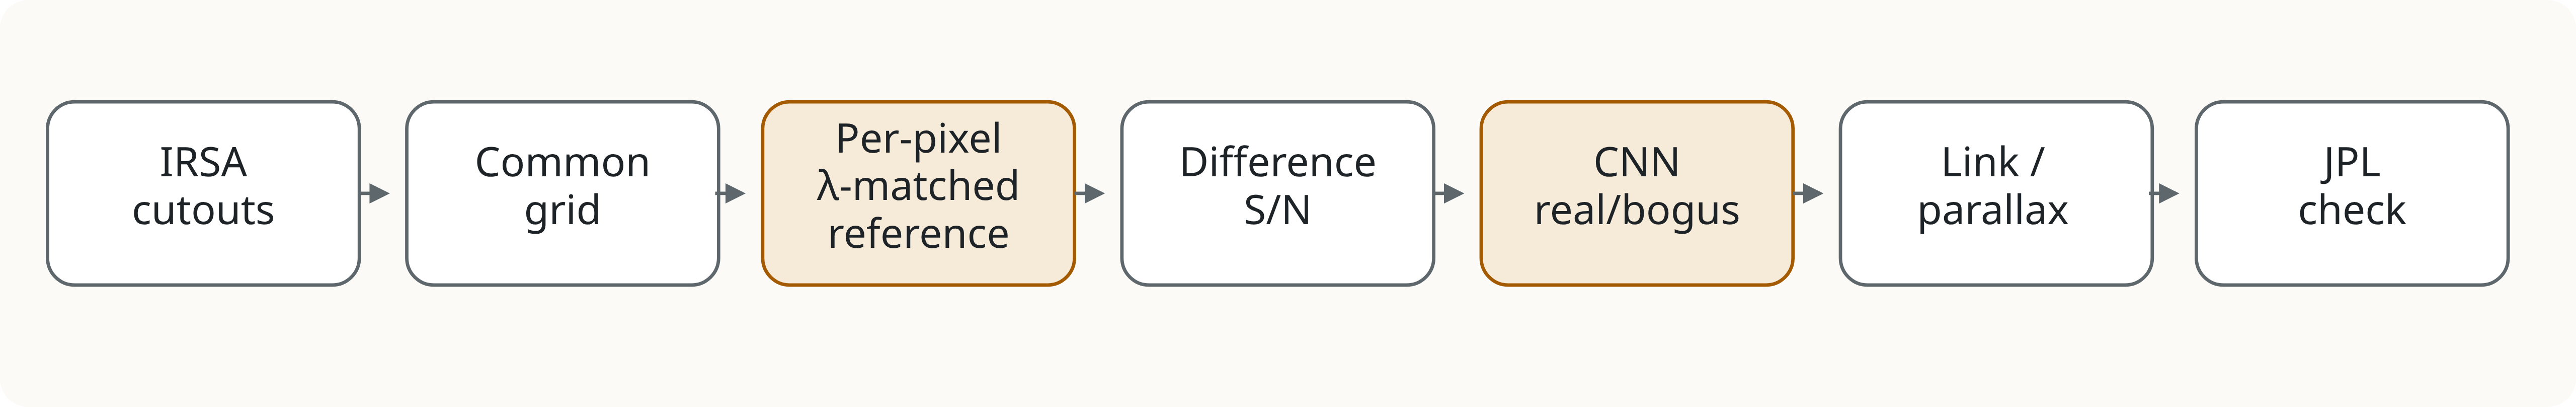
\includegraphics[width=\columnwidth]{svgfig1.png}
\caption{Pipeline. Highlighted steps are specific to SPHEREx (wavelength-matched references) or learned (CNN).}
\end{figure}
\subsection{Alignment and wavelength-matched references}
Each cutout is resampled (bilinear) onto a gnomonic grid with 6.15$''$ pixels; the coverage mask is eroded by 3 px and pixels with hard-bad flags (transient, overflow, hot, persistence, non-linearity, bloom, halo, \ldots{}) are masked. For exposure \emph{i}, the reference at every pixel is the median of exposures \emph{j} of the same detector with |t\textsubscript{j} $-$ t\textsubscript{i}| $\ge$ 3 h and |$\lambda$\textsubscript{j} $-$ $\lambda$\textsubscript{i}| $\le$ 0.03 $\lambda$\textsubscript{i} \emph{at that pixel}. Across a 0.5$^\circ$ cutout the filter wavelength changes by about 7\%, so a single wavelength per image would mix colours. With a 2\% tolerance, 95\% of exposures in a test field had at least two reference images.

\subsection{Difference image and noise model}
$\alpha$ is the median of I/R over pixels where the reference S/N exceeds 30 (it ranged 0.83--1.13), $\sigma$\textsubscript{R}\textsuperscript{2} = ($\pi$/2) mean($\sigma$\textsubscript{j}\textsuperscript{2})/n for n $\ge$ 3 references, and $\varepsilon$ = 0.1. The last term absorbs star residuals caused by the undersampled PSF. It must use the reference flux only: a first version used max(I, R), which capped every bright real mover at S/N $\approx$ 1/$\varepsilon$ = 10 (Section 5.1). Local maxima with S/N $\ge$ 5 become candidates.

\subsection{Injections}
Synthetic sources are added to the native-frame image before resampling, using the PSF of the nearest detector zone, shifted by the sub-pixel offset and binned from the 10$\times$ oversampled grid. Per field we injected 60 linear movers (AB 14--21.5 uniform, 1--150$''$/h log-uniform, random direction, active for up to 4 d) and 3 distant bodies (150--800 AU, fixed barycentric position; their apparent motion is Earth's parallax). Injected flux is added without its own Poisson noise.

\subsection{Real/bogus network}
Each candidate becomes a 4 $\times$ 21 $\times$ 21 stamp: image, reference and S/N in noise units (compressed with asinh(x/3)), plus a mask of catalogued-source and ghost flags. We deliberately left out the pipeline's \texttt{MP\_OUTLIER} flag: it is set on real movers but never on injected ones, so a network could learn it as a simulation-only shortcut. The network has three convolutional blocks (32/64/128 channels), mean-and-max pooling and a small MLP (321,505 parameters), trained with class-weighted binary cross-entropy, AdamW, a one-cycle schedule, 90$^\circ$ rotations and flips, for 30 epochs. Splits are by field: 12 training, 2 validation (\texttt{ecl120+00}, \texttt{ecl315-12}), 2 test (\texttt{ecl180+00}, \texttt{ecl060+00}). Probabilities are temperature-scaled on validation (T = 0.780), and the operating threshold is fixed on validation at 1\% FPR.

\subsection{Linking}
\emph{Distant bodies first.} Within each survey pass we group $\ge$ 3 confident detections (p $\ge$ 0.5) that lie within 8$''$ of each other in $\ge$ 2 epochs. Between passes a distant body moves by Earth's parallax \emph{and} by its own orbital motion, which at a few hundred AU is as large as the parallax ($\approx$ 150$''$/yr at 420 AU). For each trial distance d (1500 log-spaced values, 30--3000 AU) we predict the parallax-only position of every other group, accept groups within reach of a bound orbit (speed $\le$ $\surd$2 $\times$ circular), fit one linear drift through them, and keep the set that leaves every group within 8$''$. At least three passes are required: with two, any offset is absorbed by some drift and distance cannot be separated from motion. At least one linked pair must be separated by $\ge$ 3 px, otherwise it is a static residual. Detections on the fitted path are then absorbed and (d, $\mu$\textsubscript{$\alpha$*}, $\mu$\textsubscript{$\delta$}) refitted. \emph{Catalogue help.} For display, detections matched to a JPL object join linking whatever their AI score; every track is also marked by whether linking on the AI score alone (blind) finds it, and Section 4.5 reports the blind numbers. \emph{Fast movers.} The remaining detections are linked within each pass as straight lines: pairs 0.5 h--3 d apart at 0.5--300$''$/h, at least 4 detections in at least 3 distinct 30-min epochs, residuals $\le$ 8$''$, and total motion $\ge$ 16$''$. These thresholds were set on the 65 Cybele field, where looser settings produced dozens of chance alignments.

\section{Results}
\label{sec:results}
\subsection{Real known asteroids (H1)}
\begin{figure}[t]
\centering
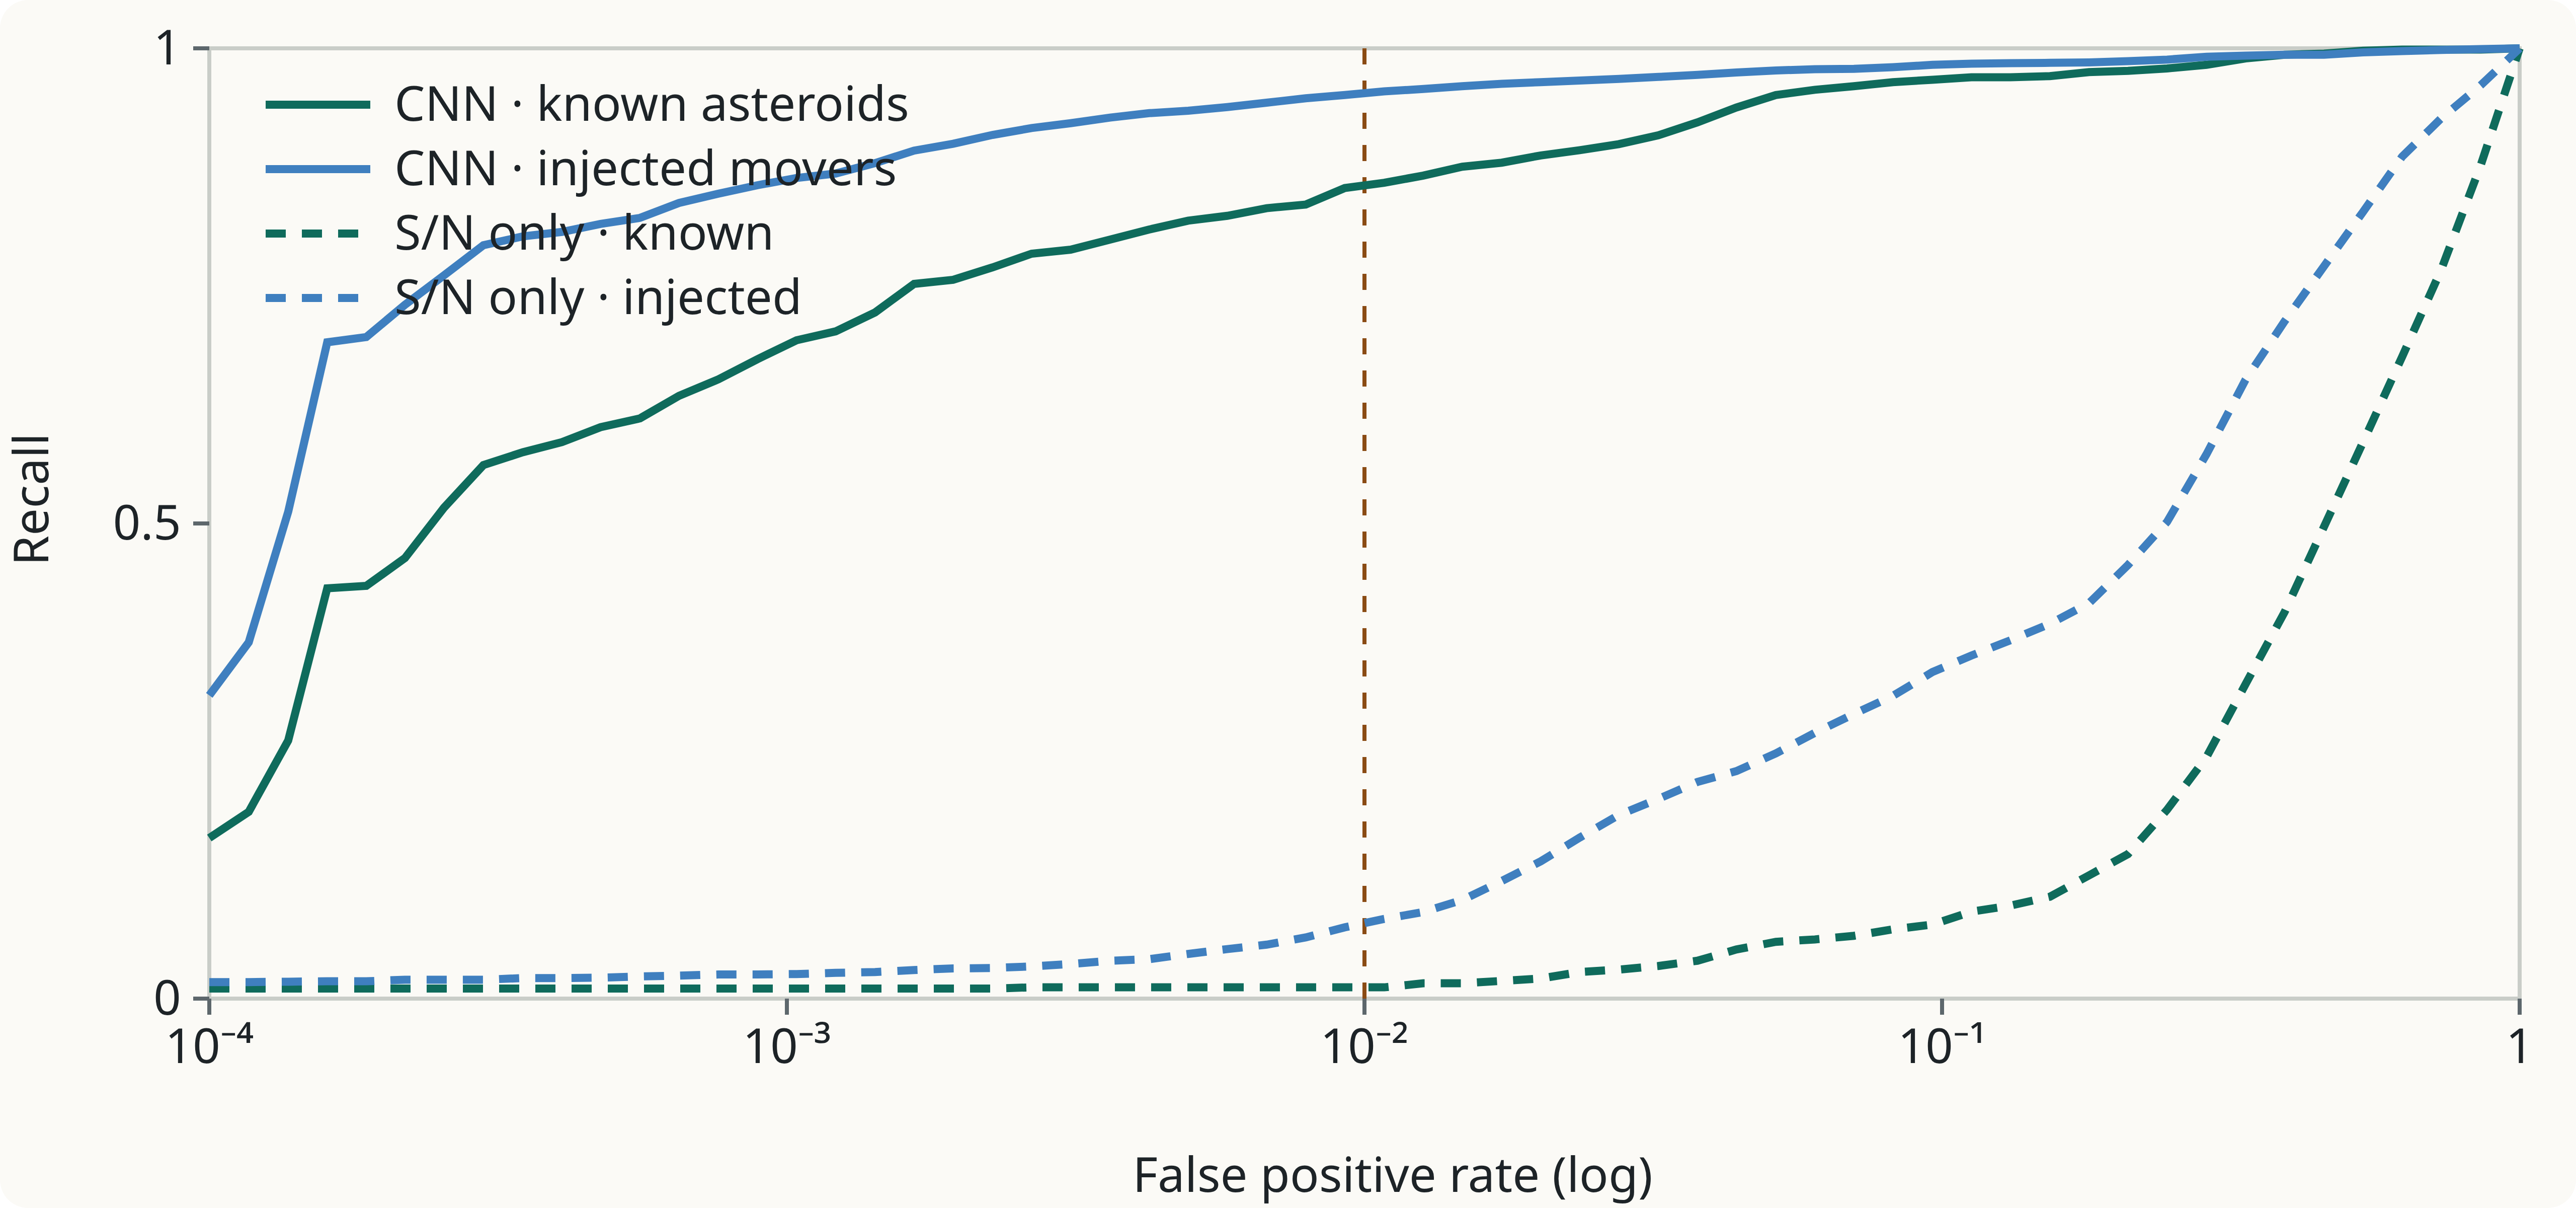
\includegraphics[width=\columnwidth]{svgfig2.png}
\caption{ROC curves. Solid: CNN; dashed: S/N of the difference image alone. Green: 755 detections of real known asteroids (V $\le$ 18.5) versus bogus candidates from the held-out test fields; blue: injected movers in the test fields. Dotted line: 1\% FPR.}
\end{figure}
The CNN reaches AUROC 0.985 (95\% CI 0.981--0.990) on real known asteroids (the asteroids themselves were never in training), and recall 85.3\% (82.6--87.6\%) at the validation threshold. The S/N of the difference image alone is no better than chance (AUROC 0.512): many artifacts, mostly star residuals, are as bright as real movers. On injected movers in the held-out fields the AUROC is 0.992 (0.989--0.994), with recall 95.1\% at FPR 0.94\%. Confidence intervals resample candidates and ignore field-to-field variance.

\emph{A cleaner comparison.} The numbers above pool known asteroids from 31 fields, 199 of whose detections lie in training-field images (the asteroids themselves were removed from training), against false signals from only the two test fields. Restricting to the 19 validation, test and benchmark fields the CNN never trained on, and drawing false signals from those same fields (380,000), gives AUROC 0.987 (0.981--0.992), recall 90.8\% at FPR 1.15\%, and S/N alone 0.537. We treat this as the headline number.

\begin{table}[t]
\centering
\footnotesize

\begin{tabular}{llll}
\hline\hline
V magnitude & n & Recall & 95\% CI \\
\hline
< 15 & 111 & 94.6\% & 88.7--97.5\% \\
15--16 & 136 & 99.3\% & 96.0--99.9\% \\
16--17 & 197 & 87.3\% & 81.9--91.2\% \\
17--18.5 & 305 & 75.4\% & 70.3--79.9\% \\
\hline
\end{tabular}
\end{table}
\subsection{False positives by detector (H2)}
\begin{table*}[t]
\centering
\footnotesize

\begin{tabular}{lllllll}
\hline\hline
Detector & Wavelength & Known n & Recall (95\% CI) & Injected recall & Bogus n & FPR \\
\hline
D1 & 0.75--1.11 $\mu$m & 176 & 79.5\% (73.0--84.8) & 92.6\% & 20,089 & 0.25\% \\
D2 & 1.10--1.64 $\mu$m & 231 & 87.9\% (83.0--91.5) & 95.7\% & 12,960 & 0.24\% \\
D3 & 1.63--2.42 $\mu$m & 122 & 85.2\% (77.9--90.5) & 95.5\% & 10,619 & 0.66\% \\
D4 & 2.40--3.82 $\mu$m & 108 & 86.1\% (78.3--91.4) & 96.1\% & 12,149 & 2.50\% \\
D5 & 3.81--4.42 $\mu$m & 70 & 87.1\% (77.3--93.1) & 93.9\% & 9,268 & 1.06\% \\
D6 & 4.41--5.00 $\mu$m & 48 & 89.6\% (77.8--95.5) & 97.2\% & 7,826 & 1.66\% \\
\hline
\end{tabular}
\end{table*}
Overall FPR meets the 1\% target, but it is not uniform: the longer-wavelength detectors produce more confident false positives. H2 as stated ($\le$ 1.5\% in every detector) is therefore not met. Detector-specific thresholds would fix the operating point, but we have not yet established why these detectors differ.

\subsection{Injection--recovery completeness}
\begin{figure}[t]
\centering
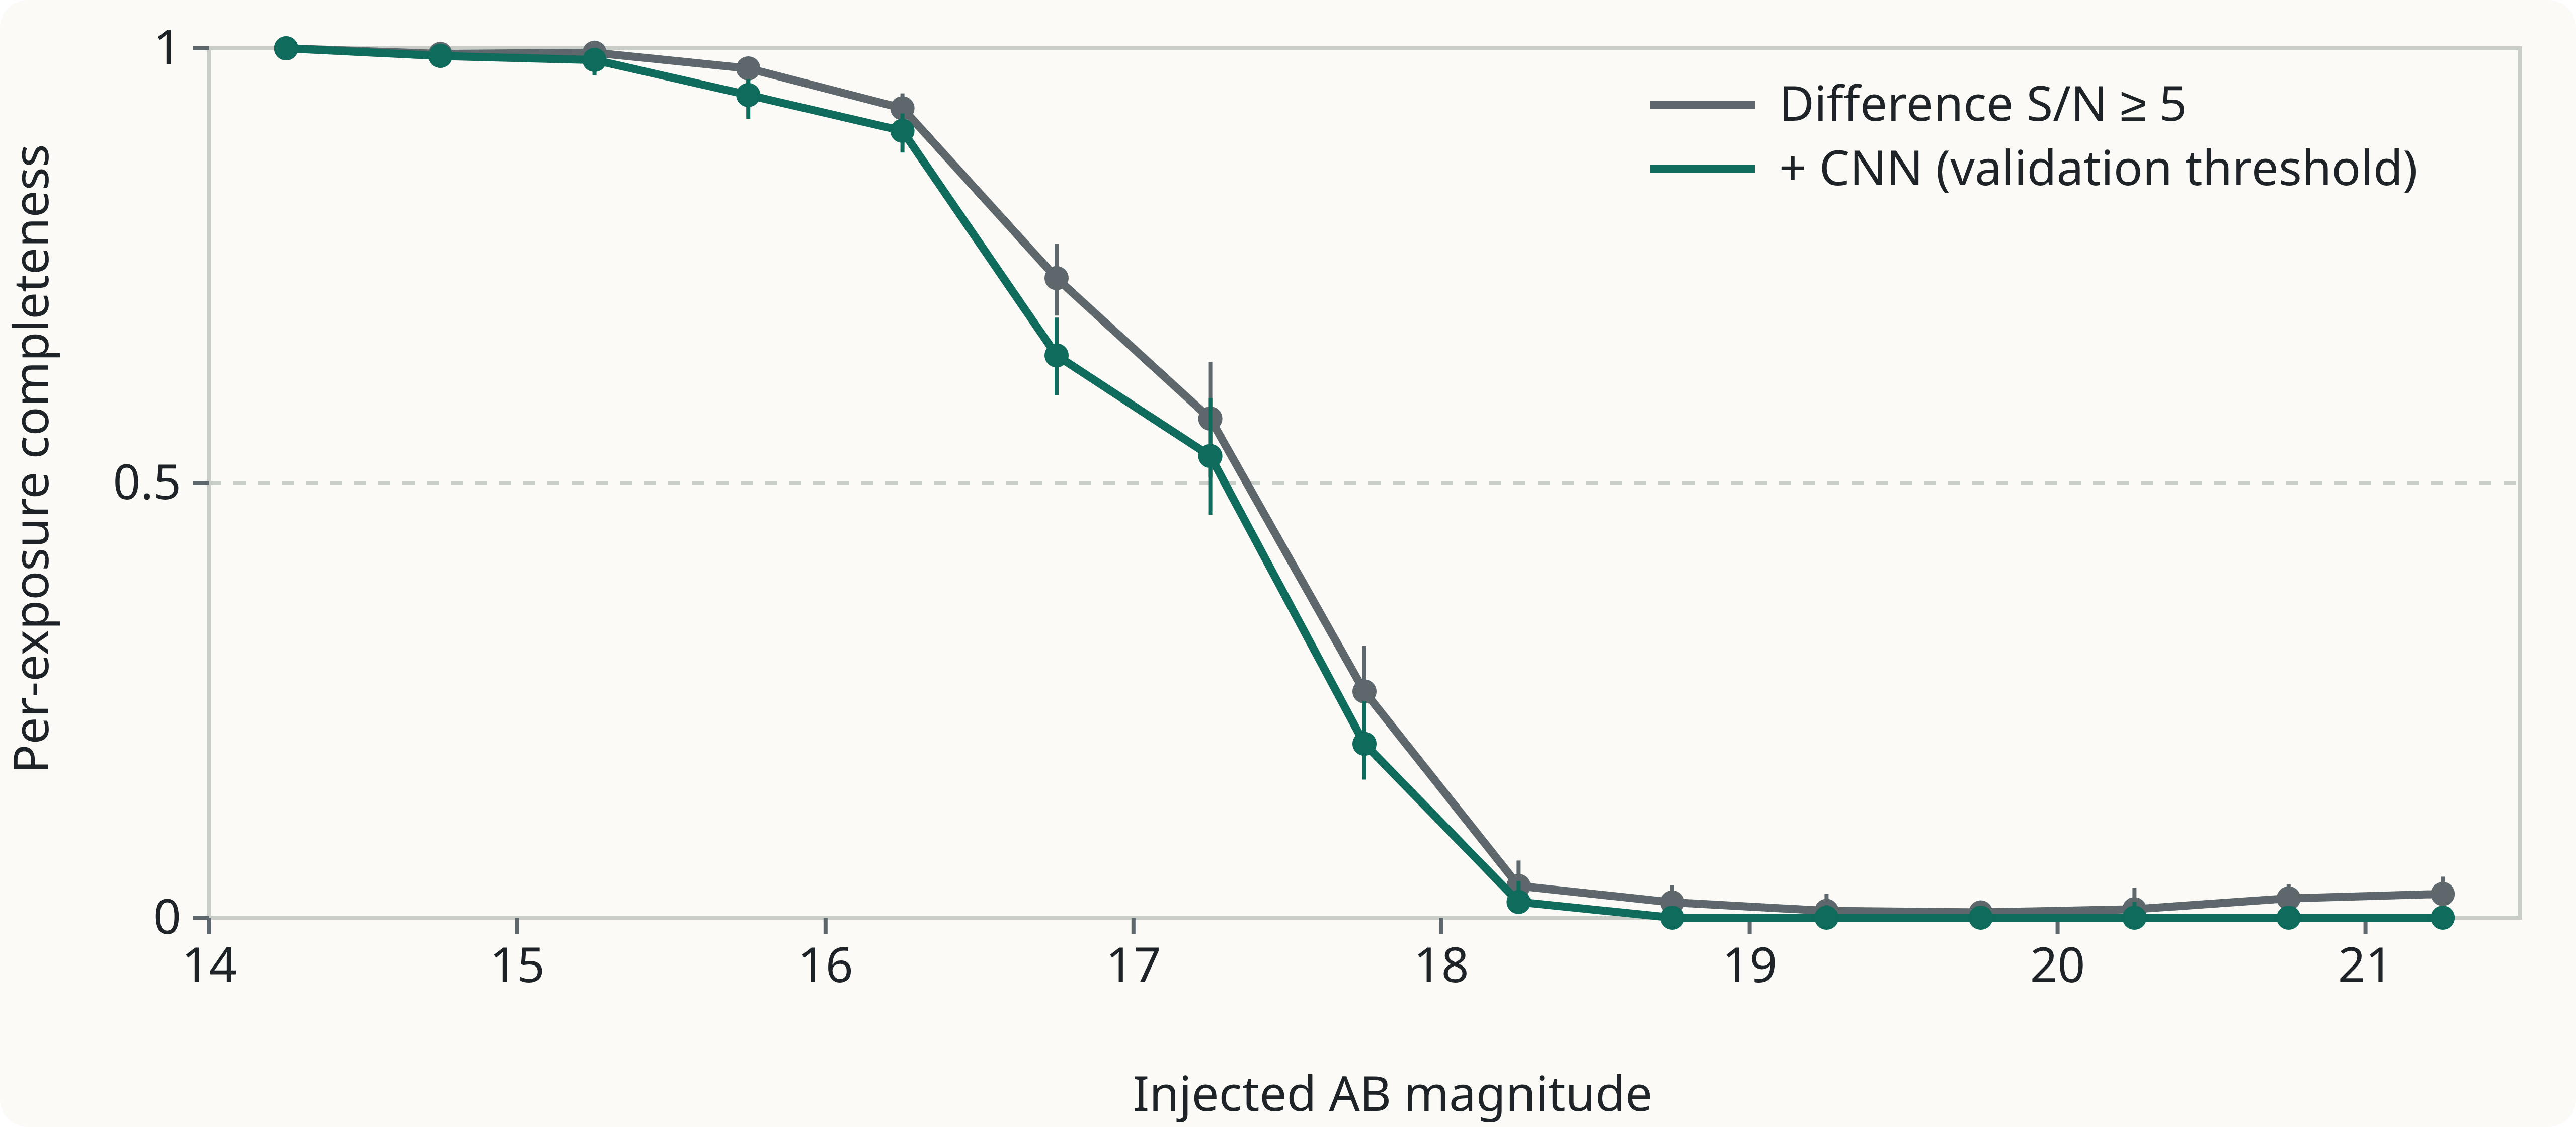
\includegraphics[width=\columnwidth]{svgfig3.png}
\caption{Per-exposure completeness for injected movers in the two test fields (Wilson 95\% intervals). The CNN removes few real sources: the curves nearly overlap.}
\end{figure}
Half of the injected movers are recovered at AB 17.3 per exposure. This is a single-exposure limit; fainter sources seen in many exposures need shift-and-stack (Section 4.8).

\subsection{Distant bodies from parallax (H3)}
\begin{table*}[t]
\centering
\footnotesize

\begin{tabular}{lllll}
\hline\hline
Distance (AU) & AB 15: recovered & AB 16: recovered & AB 17: recovered & Median distance error \\
\hline
500 & 4/5 & 4/5 & 4/5 & 0.02\% \\
800 & 4/5 & 4/5 & 3/5 & 0.04\% \\
1500 & 4/5 & 4/5 & 4/5 & 0.09\% \\
3000 & 4/5 & 4/5 & 4/5 & 0.23\% \\
\hline
\end{tabular}
\end{table*}
47 of 60 injected bodies were recovered, with a median distance error of 0.09\% and a maximum of 37.55\%. The search also produced 0 distant-body tracks that matched no injection, in 0 of the 5 fields; in a real search each would need follow-up. Every injected body moves on a circular orbit in a random direction, and the fitted orbital motion differs from the injected one by a median 0.8$''$/yr. By field: in the 4 fields with three survey passes 47/48 bodies were recovered; the 1 field with only two passes recovered 0/12, as it must, because with two passes any offset is absorbed by some orbital drift. 1 recovered bodies have distance errors above 1\% (up to 38\%): there the fit settled on the wrong combination of distance and motion, which a fourth pass would break. An earlier version of this test injected bodies with no orbital motion and fitted the same model; it recovered 59/60 at 0.15\% median error, but that only showed the code agreeing with its own simulation.

\subsection{Case studies}
\textbf{65 Cybele.} In the Virgo field, the pipeline linked 24 detections of 65 Cybele at 24.9$''$/h (JPL gives 24$''$/h). The field shows 7 tracks, but 3 of them were only linked with catalogue help; blind linking on the AI score finds 4 tracks, 3 of them known asteroids. Checking every named track against JPL, 4 agree and 2 picked up unrelated detections (the web tool marks them). \textbf{Simulated planet.} A body injected at 420.0 AU (AB 15.5) into real images was recovered as one track of 327 detections over 4 passes at 420.2 AU.

\begin{figure*}[t]
\centering
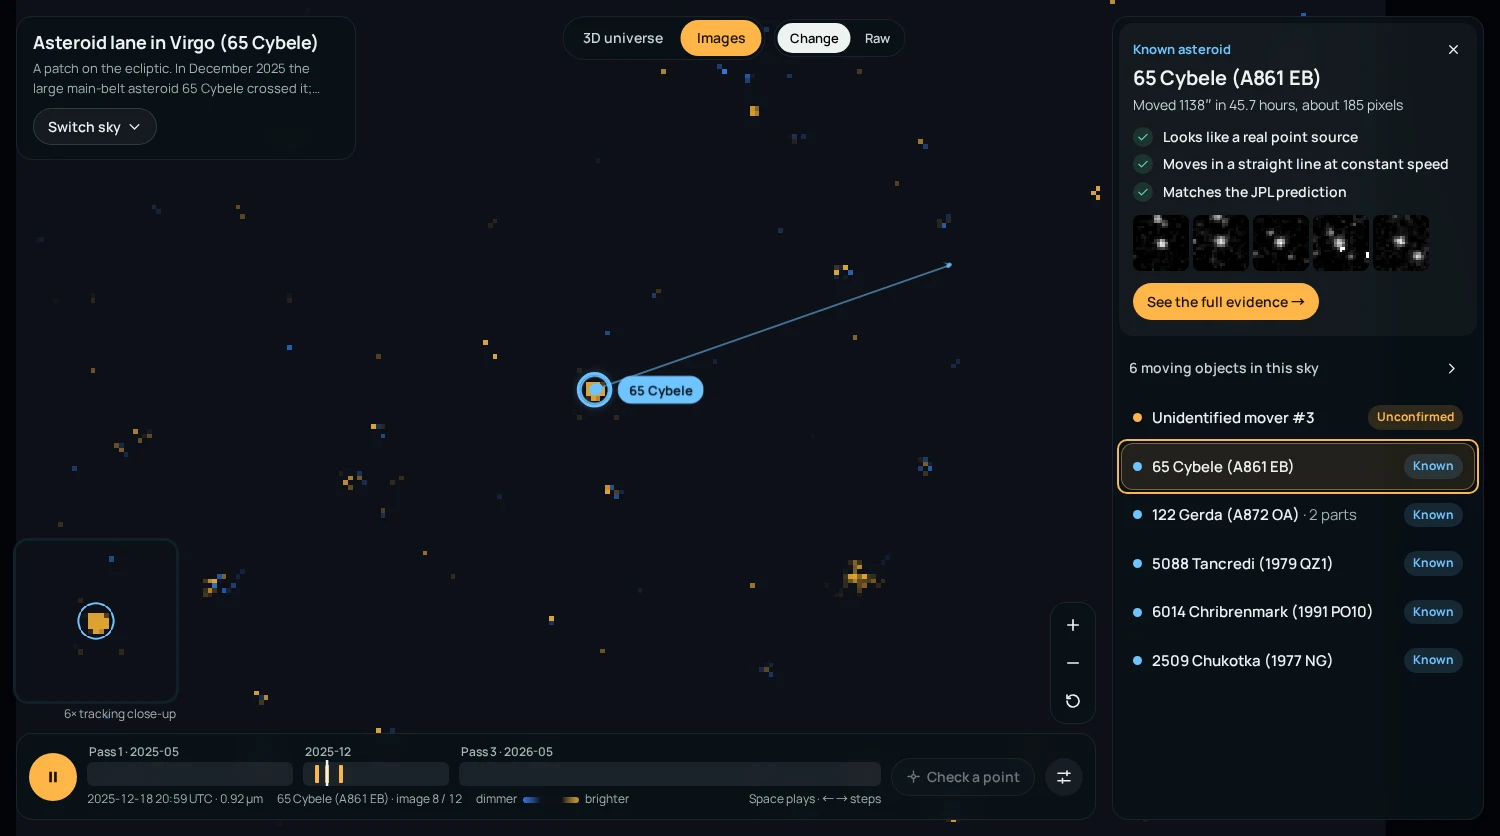
\includegraphics[width=0.95\textwidth]{img_viewer_en.png}
\caption{The public viewer: the difference image (amber = brighter than the reference) while following 65 Cybele.}
\end{figure*}
\subsection{Astrometry against JPL, seen from SPHEREx}
For every track named after a known object we asked JPL Horizons for the object's astrometric position at each detection time with the SPHEREx spacecraft (Horizons ID $-$163182) as observer; from low Earth orbit the observer position alone moves a main-belt asteroid by up to \textasciitilde{}5$''$. In tracks whose detections agree with JPL, 78 detections of 6 objects lie a median 0.7$''$ from the prediction (0.11 of a 6.15$''$ pixel; 90th percentile 1.47$''$). 3 named tracks had a quarter or more of their detections far from JPL and are flagged as mixed rather than counted.

\subsection{Distances of real dwarf planets}
Parallax carries a trans-Neptunian dwarf planet 1--2$^\circ$ across the sky in half a year, more than one field, so we opened one 0.6$^\circ$ field per survey pass centred on the JPL ephemeris, ran the same pipeline, and merged the AI candidates of the three passes (score $\ge$ P\_LINK, no catalogue) for the distant-body search. \textbf{Makemake}: the blind search links exactly one distant track in all of the data, and it is Makemake (56 detections, three passes), at 52.71 AU against JPL's 52.72 AU (0.02\% off). \textbf{Haumea}: again one track, 49.49 AU against 49.82 AU (0.66\%). \textbf{Eris} (95.52 AU, V $\approx$ 18.7) is not detected in single exposures, and shift-and-stack did not recover it either: within the two weeks of one pass its own orbital motion moves it about 9 pixels, while our stacking only compensates parallax (it is built for bodies beyond 150 AU that barely move). To link Makemake this close in, the linker gained slow tracklets and a curvature allowance; in fields holding twelve distant bodies at once that version mixed different bodies, and the grid of Section 4.4 briefly regressed to 45 false tracks. Building same-position groups first, forming tracklets only from what is left, and requiring every detection of a link to lie on one path restored 0 false tracks and a median distance error of 0.09\% (Table 4 shows the fixed version).

\subsection{Shift-and-stack}
For each pass and 36 trial distances (40--3000 AU), the difference S/N images are shifted along the predicted parallax path back to the pass mid-time and added. The first version added raw S/N, recovered 3/36 injected bodies and produced about 800 false tracks: single difference images have heavy noise tails (1.3\% of pixels above 3$\sigma$, from asteroids, cosmic rays and subtraction residuals) that pile up into false stacked peaks, which then also steal the real body's peaks during linking. Now each frame is clipped at $\pm$3$\sigma$ (a faint body is \textasciitilde{}1$\sigma$ per frame and is unaffected), each stack is divided by its own robust noise, the link tolerance is 4$''$, and every linked peak is re-stacked at the track's distance to confirm it. Injecting AB 18--20.5 bodies at 500 and 1500 AU into three uncrowded fields never used for training: 14/18 recovered at AB 18--19 and 0/18 at AB $\ge$ 19.5, a 50\% completeness of about AB 19.2, about 2 mag deeper than single exposures, with 0 false tracks.

\subsection{A search along the predicted path of Planet Nine}
Following the sky path of the Brown \& Batygin (2021) median orbit and the regions Brown et al. (2024) left unexcluded, we took one 0.5$^\circ$ field every 1.5$^\circ$ along the path in region A (RA 75--105$^\circ$, the northern galactic-plane crossing) and region B (RA 45--74$^\circ$, near aphelion), plus a 3$\times$3 grid around the 2025 IRAS/AKARI candidate of Phan et al. (2025) extrapolated to 2025 (region D), keeping only fields with at least three survey passes: A 3, B 20, D 9, 7.89 deg$^2$ after the star mask. This samples the path; it does not cover the whole $\pm$12$^\circ$ probability band.

\emph{Single exposures.} The distant-body search linked no track in any of the 32 fields (0). \emph{Stacking.} It linked 63 tracks, concentrated in the most crowded fields nearest the galactic plane. After per-track checks (three passes, fit residual, bound orbit, not static, distance not at the edge, JPL known objects, consistent brightness across passes), 23 were rejected for inconsistent brightness and 1 for coinciding with a known asteroid, and 39 passed all of them. To estimate chance, we cyclically relabelled the pass times and linked and confirmed again, which no real body can survive: 55 and 60 tracks (mean 57.5), against 63 with the true times, a difference within Poisson scatter. As a set, these tracks cannot be told apart from chance alignments in crowded fields, and we list none of them as a candidate.

\emph{Limit.} In these 7.89 deg$^2$ there is no body brighter than about AB 17 at 30--3000 AU, and down to AB 19.2 nothing that stands out from chance. The stacking completeness was measured in uncrowded fields; it is lower near the galactic plane. Applying the predicted brightness of Planet Nine (V = 22.0 +1.1/$-$1.4, Brown et al. 2024) only roughly, about 2.3\% of cases would be brighter than AB 19.2 (its near-infrared colour is unknown and methane would make it fainter), so this non-detection is expected and places almost no constraint on Planet Nine.

\section{Discussion}
\label{sec:discussion}
\subsection{Closing the simulation-to-real gap}
Our first evaluation on "known asteroids" gave AUROC 0.66. Three separate problems were behind it, and only one was the network. (1) \emph{Labels.} Most matched "known" objects had V $\approx$ 20, far below what one exposure can show; their predicted positions fell on star residuals by chance. We now count only V $\le$ 18.5 objects matched within 1.5 px, and we added bright-asteroid fields. (2) \emph{Noise model.} The systematic term used max(I, R) and capped bright real movers at S/N $\approx$ 10. (3) \emph{Shortcut.} The level-2 pipeline sets \texttt{MP\_OUTLIER} on real moving sources; injections never have it. Removing it from the input forces the network to learn morphology. We now show the flag in the web tool as independent evidence.

\subsection{Limitations}
\begin{itemize}
\item QR3 injections use a QR2 PSF cube; injected sources add no Poisson noise.
\item Known-object positions are propagated linearly for up to 0.25 d; faint-end recall may be underestimated.
\item Confidence intervals resample candidates, not fields; with two test fields, between-field variance is not captured.
\item Linking thresholds were tuned on two of the fields that also appear as case studies.
\item Per-detector false-positive rates differ by an order of magnitude (Table 3).
\item The demo planet is deliberately bright (AB 15.5). A real distant planet would be far fainter than our single-exposure limit.
\item Shift-and-stack compensates parallax only and does not search orbital motion; bodies within \textasciitilde{}150 AU (e.g. Eris) smear within a pass. Its completeness was measured in uncrowded fields.
\item The chance estimate of Section 4.9 uses only two time relabellings; the survey samples the predicted path, not the whole probability band.
\item Orbital motion is modelled as a linear drift over the \textasciitilde{}1-year baseline, adequate beyond \textasciitilde{}100 AU but not for closer objects.
\item The tracks shown on the website include catalogue-assisted links; the blind numbers in Section 4.5 are the pipeline's own performance.
\item The known-asteroid AUROC in Figure 2 pools positives from training-field images with negatives from two test fields; the same-field comparison in Section 4.1 is cleaner.
\end{itemize}

\subsection{What finding Planet Nine would still need}
Single exposures (about AB 17) and shift-and-stack (about AB 19.2) are both more than 3 mag shallower than the predicted V $\approx$ 22 of Planet Nine. Going deeper needs combining the bands of a pass into a broad band (hundreds of exposures per body), searching orbital motion inside the stack, and more passes (SPHEREx adds one every six months; a fourth breaks the distance--motion degeneracy). Crowding is the other bottleneck: the chance rate of Section 4.9 shows that near the galactic plane better star subtraction is needed before real signals can stand out. Any candidate must be confirmed by follow-up with larger telescopes and reported under the MPC's rules (SPHEREx is observatory code 288).

\section{Conclusions}
\label{sec:conclusions}
Wavelength-matched differencing makes SPHEREx usable for change detection. A network trained only on simulations transfers to real asteroids once labels, the noise model and a pipeline-flag shortcut are fixed. Fitting parallax and orbital motion together recovers injected distant bodies on realistic orbits, given three or more survey passes, and measures the distances of real dwarf planets to within 1\% from SPHEREx parallax alone. A search along the predicted path of Planet Nine found nothing that stands out from chance and sets a brightness limit for that sky. The public tool shows people the result of these measured steps rather than raw blinking images.

\section*{Open research}
Code (pipeline, training, evaluation and web app) is in the project repository under \texttt{spherex/}. SPHEREx images are public at NASA/IPAC IRSA; known-object data come from the JPL SSD APIs. Every number in this paper is generated by \texttt{scripts/build\_paper\_evidence.py} and \texttt{scripts/render\_paper.py} from the files below. The hashes show that these files are unchanged since rendering, not when they were created. The released network (\texttt{/models/rb\_cnn.pt}) and its metrics are public; training checkpoints and raw score dumps are not served.

\begin{table}[t]
\centering
\footnotesize

\begin{tabularx}{\columnwidth}{Xl}
\hline\hline
File & SHA-256 (first 12) \\
\hline
\texttt{paper\_evidence/evidence.json} & \texttt{e145327c9a66} \\
\texttt{models/metrics.json} & \texttt{3fba3faee765} \\
\texttt{models/recovery.json} & \texttt{f802fbe4a5c4} \\
\texttt{models/rb\_cnn.pt} & \texttt{eca4e82ba7de} \\
\texttt{paper\_evidence/planetx\_grid.json} & \texttt{0d9835794331} \\
\hline
\end{tabularx}
\end{table}
Evidence files: evidence.json $\cdot$ planetx\_grid.json $\cdot$ metrics.json $\cdot$ recovery.json.

\textbf{Data credits.} This work uses data from SPHEREx, a NASA mission, obtained through the NASA/IPAC Infrared Science Archive, and the JPL Small-Body Identification API. It is a hackathon prototype and is not endorsed by NASA.

\section*{Appendix}
\subsection*{A. Hypotheses, criteria and deviations}
\begin{table*}[t]
\centering
\footnotesize

\begin{tabularx}{\textwidth}{lXXXl}
\hline\hline
Hypothesis & Criterion & When it was set & Result & Met? \\
\hline
H1 & Real known-asteroid AUROC $\ge$ 0.95 and recall $\ge$ 80\% at 1\% FPR & 2026-10-20, before training (PLAN.md G3) & AUROC 0.985 (0.981--0.990); recall 85.3\% (82.6--87.6\%) & Met \\
H2 & FPR $\le$ 1.5\% in every detector (validation threshold) & 2026-10-21, after seeing the overall FPR (post hoc) & 0.94\% overall; D2 0.24\% -- D4 2.50\% & Not met \\
H3 & Distance error of injected distant bodies $\le$ 2\% & 2026-10-21, before the injection grid was run (WEB\_PAPER\_PLAN.md) & 47/60 recovered; median 0.09\%, max 37.55\% & Partly met \\
\hline
\end{tabularx}
\end{table*}
\textbf{Deviations from the original plan.} (a) The bright-asteroid benchmark was stopped at 15 of 20 fields to save compute. (b) The known-label magnitude limit was changed from V $\le$ 21.5 to V $\le$ 18.5 after inspecting an early run. (c) The outlier-flag channel was removed and the noise model corrected after that run; the network was then retrained from scratch. (d) Track-linking thresholds were set on demonstration fields.

\subsection*{B. Settings}
Field size 0.5$^\circ$ (0.3$^\circ$ for fields analysed on request); cutout 1.5$\times$ field; reference: $\le$ 36 candidate exposures, 3\% wavelength tolerance, $\ge$ 3 h separation; $\varepsilon$ = 0.1; detection S/N $\ge$ 5, 5 $\times$ 5 local maximum; stamps 21 px; training 30 epochs, batch 512, learning rate 10\textsuperscript{$-$3}, positive weight $\le$ 20; linking tolerance 8$''$, p $\ge$ 0.5.

\section*{Acknowledgements}
This publication makes use of data products from the Spectro-Photometer for the History of the Universe, Epoch of Reionization and Ices Explorer (SPHEREx), which is a joint project of the Jet Propulsion Laboratory and the California Institute of Technology, and is funded by the National Aeronautics and Space Administration. This work has made use of the NASA/IPAC Infrared Science Archive, which is funded by the National Aeronautics and Space Administration and operated by the California Institute of Technology (SPHEREx DR1, doi:10.26131/IRSA678; QR3, doi:10.26131/IRSA662; QR2, doi:10.26131/IRSA652). This work has made use of data from the European Space Agency (ESA) mission Gaia, processed by the Gaia Data Processing and Analysis Consortium (DPAC); funding for the DPAC has been provided by national institutions, in particular the institutions participating in the Gaia Multilateral Agreement.

\section*{References}
\begin{list}{}{\leftmargin=1.5em\itemindent=-1.5em\itemsep=2pt\small}
\item Astropy Collaboration et al. (2022). The Astropy Project: sustaining and growing a community-oriented open-source project. \emph{ApJ}, 935, 167.
\item Batygin, K., \& Brown, M. E. (2016). Evidence for a distant giant planet in the Solar System. \emph{AJ}, 151, 22.
\item Brown, M. E., \& Batygin, K. (2021). The orbit of Planet Nine. \emph{AJ}, 162, 219.
\item Brown, M. E., Holman, M. J., \& Batygin, K. (2024). A Pan-STARRS1 search for Planet Nine. \emph{AJ}, 167, 146.
\item Phan, T. L., Goto, T., et al. (2025). A search for Planet Nine with IRAS and AKARI data. \emph{PASA}; arXiv:2504.17288.
\item Minor Planet Center. Reporting observations (ADES) and observatory codes. https://docs.minorplanetcenter.net/
\item Doré, O., et al. (2014). Cosmology with the SPHEREX all-sky spectral survey. arXiv:1412.4872.
\item Duev, D. A., et al. (2019). Real-bogus classification for the Zwicky Transient Facility using deep learning. \emph{MNRAS}, 489, 3582.
\item Guo, C., Pleiss, G., Sun, Y., \& Weinberger, K. Q. (2017). On calibration of modern neural networks. \emph{ICML}.
\item Kuchner, M. J., et al. (2017). The first brown dwarf discovered by the Backyard Worlds: Planet 9 citizen science project. \emph{ApJL}, 841, L19.
\item NASA/IPAC Infrared Science Archive. SPHEREx Quick Release data and image-cutout service documentation.
\item JPL Solar System Dynamics. Small-Body Identification API (sb\_ident).
\end{list}

\end{document}
